%\documentclass[margin=10pt]{standalone}
%\usepackage{pgfplots}
\pgfplotsset{compat=1.13}% <- immer compat setzen!
\usepgfplotslibrary{fillbetween}
%\begin{document}
	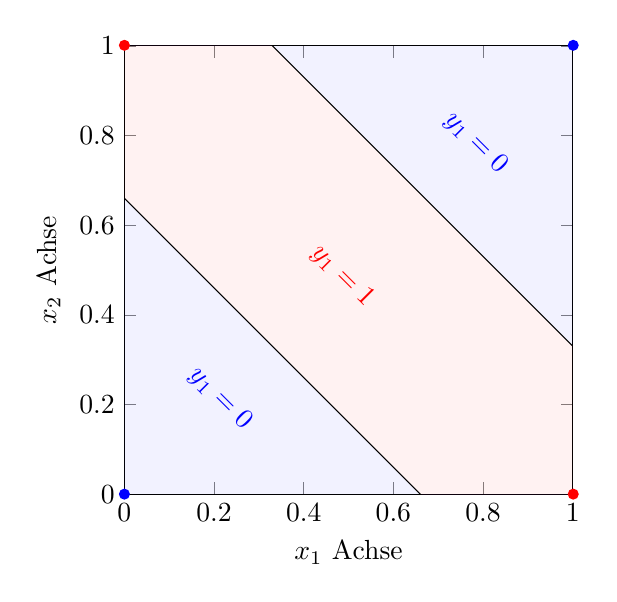
\begin{tikzpicture} 
	\begin{axis}[
	domain=0:1,% geändert
	ymin=0, ymax=1,
	xmin=0, xmax=1,
	axis equal image,
	xlabel = $x_1$ Achse,
	ylabel = $x_2$ Achse
	]

	\path[name path=axisy] (0,1) -- (1,1);
	\path[name path=axisx] (0,0) -- (1,0);

	\addplot+[mark=none, color=black, name path=A] {0.66-\x}
		node[above, color= blue, rotate=-45] at (0.75,0.75) {$y_1=0$}
		node[above, color= blue, rotate=-45] at (0.18,0.18) {$y_1=0$}
	;
	\addplot+[mark=none, color=black, name path=B] {1.33-\x} 
		node[below, color=red, rotate=-45] at (0.52,0.52) {$y_1=1$}
	;
	
	\addplot [blue,fill opacity=0.05]
	fill between[of=A and axisx]
	;
	\addplot [blue,fill opacity=0.05]
	fill between[of=B and axisy]
	;
	
	\addplot [red,fill opacity=0.05]
		fill between[of=A and B]
	;
	    

	\end{axis} 
	
	\coordinate (a) at (0,0);
	\fill[blue] (a) circle (2pt);
	\coordinate (b) at (5.7,5.7);
	\fill[blue] (b) circle (2pt);
	
	\coordinate (c) at (0,5.7);
	\fill[red] (c) circle (2pt);
	\coordinate (d) at (5.7,0);
	\fill[red] (d) circle (2pt);
	
	\end{tikzpicture}
%\end{document}